\documentclass{article}
\usepackage{amsmath,amssymb}
\usepackage{caption} % can suppress numbering of tables or figures
\usepackage{float} % for [H] placement of floats
\usepackage[utf8]{inputenc}
\usepackage{enumitem}
\usepackage{biblatex}  
\usepackage{array}  
\usepackage{hyperref}
\usepackage{graphicx}
\usepackage{subcaption}
\usepackage[table]{xcolor}


\setlength{\parskip}{0.4em}
\graphicspath{ {./images/} }

\hypersetup{
    colorlinks=true,
    linkcolor=blue,
    anchorcolor=blue,
    citecolor=blue,
    filecolor=blue,      
    urlcolor=blue,
}

\addbibresource{Assignment1.bib}

\DeclareMathOperator{\EX}{\mathbb{E}}% expected value

\begin{document}
\begin{titlepage} % Suppresses displaying the page number on the title page and the subsequent page counts as page 1
	\newcommand{\HRule}{\rule{\linewidth}{0.5mm}} % Defines a new command for horizontal lines, change thickness here
	
	\center % Centre everything on the page
	
	
	%------------------------------------------------
	%	Headings
	%------------------------------------------------
	\textsc{\Large Machine Learning}\\[0.5cm] % Major heading such as course name
	
	\textsc{\large CSI 5155}\\[0.5cm] % Minor heading such as course title
	%------------------------------------------------
	%	Title
	%------------------------------------------------
	
	\HRule\\[0.4cm]
	{\huge\bfseries Classification of Online Shoppers Purchasing Intention}\\[0.4cm] % Title of your document
	{\bfseries Assignment 1}\\[0.2cm]
	
	\HRule\\[1.5cm]
	
	%------------------------------------------------
	%	Author(s)
	%------------------------------------------------
	
	\begin{minipage}[t]{0.5\textwidth}
		\begin{flushleft}
			\large
			\textit{Authors}\\
			Alexandra \textsc{Sklokin} {\small(300010511)}\\
		\end{flushleft}
	\end{minipage}
	~
	\begin{minipage}[t]{0.4\textwidth}
		\begin{flushright}
			\large
			\textit{Professor}\\
			Dr. Herna \textsc{Viktor} % Supervisor's name
		\end{flushright}
	\end{minipage}
\vfill


	
	%------------------------------------------------
	%	Date
	%------------------------------------------------
	
	\vfill\vfill\vfill % Position the date 3/4 down the remaining page
	
	{\large\today} % Date, change the \today to a set date if you want to be precise

	\vfill % Push the date up 1/4 of the remaining page
	
\end{titlepage}

\tableofcontents
\newpage

\section{Introduction}

The purpose of this assignment is to perform an exploration to find the best model for the classification problem on online shopping data. The target feature is a boolean variable \emph{Revenue} which represents whether a client completes or abandons their online purchase. The classifiers to be trained are K-nearest neighbors (KNN), Support Vector Machine (SVM), Decision Tree, and Random Forest. 

The following report documents my methodology, and results for this assignment. Sections marked with a letter, for example (a), correspond to a requirement in the assignment instructions.

\section{Dataset}

The \emph{online\_shoppers\_intension} dataset contains 12,330 entries in 18 attributes (10 categorical and 7 numerical), one of which is the target feature \emph{Revenue}. This is a unbalanced classification problem, as 84.5\% (10,422) of the dataset is of the negative class (False), meaning that these clients did not complete their purchase. The remaining 1,908 entries belong to the positive class (True), indicating these users did complete their purchase.

\section{Methodology}

For this assignment I used \emph{jupyter notebooks}, Excel spreadsheets, and the \emph{sklearn Python} library.

Please find all of the code for this assignment in my git repository\footnote{https://github.com/alexandrasklokin/CSI5155/tree/main/Assignment1}.

\section{Preprocessing (a)}

\subsection{Cleaning the Data}

In this dataset, none of the entries are \emph{null} or unknown, therefore I did not need to clean the data. All 12,330 entries of the data were used for this experiment.

\subsection{Feature Selection}

I did not begin this assignment by feature transformations, as described in the assignment document, since 1-of-C coding of the categorical features would have increased the dimensionality of the dataset. Instead, I began by performing feature selection, and then was able to proceed with feature transformations. 

\subsubsection{SelectKBest}

My first step was to use \emph{SelectKBest} from the \emph{sklearn} library to find the best ten features. The following features were selected by the algorithm (in no particular order):

\begin{itemize}
\item \emph{Administrative, Administrative\_Duration, Informational	Informational\_Duration, ProductRelated, ProductRelated\_Duration, PageValues, SpecialDay, Month, VisitorType}
\end{itemize}

\subsubsection{Correlation Matrix}

I proceeded by using the correlation matrix (refer to Table \ref{tab:correlationMatrix}) to determine which pairs of features were most correlated. I found very high correlation (absolute values greater than 0.5) between the following pairs of features:
\begin{itemize}
  \item \emph{ExitRates} and \emph{BounceRates} (0.91)
  \item \emph{ProductRelated} and \emph{ProductRelated\_Duration} (0.86)
  \item \emph{Administrative} and \emph{Administrative\_Duration} (0.6)
\item \emph{Informational} and \emph{Informational\_Duration} (0.62)
\end{itemize}

Again using the correlation matrix, I now ranked the features, based on which were most correlated to the target feature \emph{Revenue}, but only selecting one of the two features from the above pairs of correlated features. For example, \emph{ExitRates} was more correlated to \emph{Revenue} than \emph{BounceRates}, therefore \emph{ExitRates} was included in the list of best features and \emph{BounceRates} was not. The following were the best features selected (ordered from most correlated to target features to least):
\begin{itemize}
\item \emph{PageValues, ExitRates, ProductRelated, Administrative, VisitorType, Informational, SpecialDay, Month, Weekend, Browser, OperatingSystems, Region, TrafficType}
\end{itemize}

\begin{figure}[h]
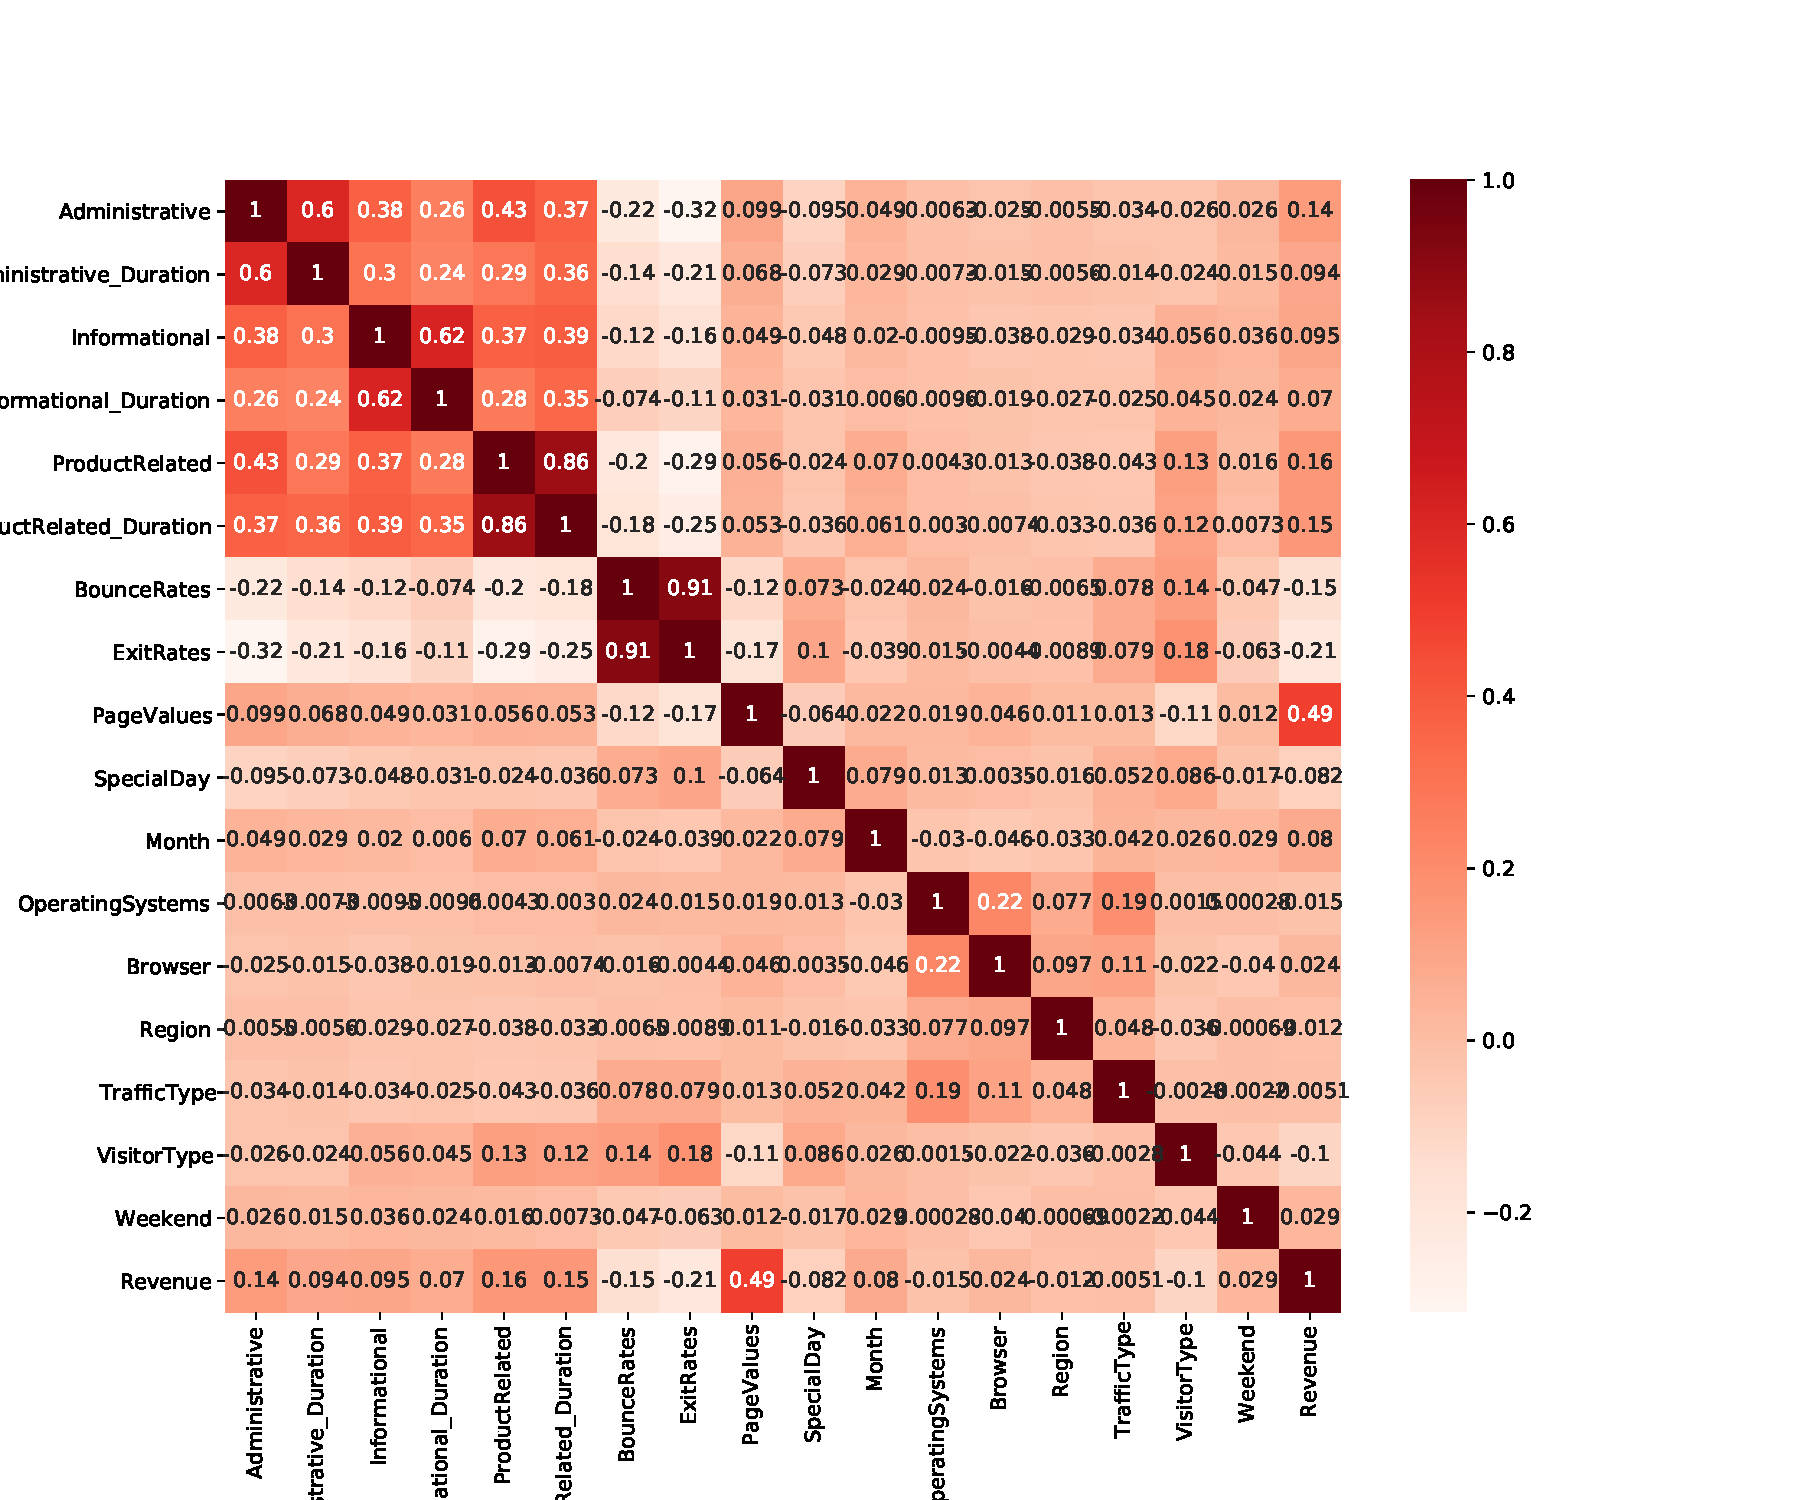
\includegraphics[width=0.95\textwidth]{correlationMatrix}
\caption{Correlation Matrix.}
\label{tab:correlationMatrix}
\end{figure}

\subsubsection{Dimension Reduction}

It turns out that the lists, generated from \emph{SelectKBest} and the correlation matrix method, have some elements in common. The \emph{SelectKBest} features include pairs of highly-correlated features, which I did not want to include for training due to the multicollinearity conundrum. Instead, I used the features selected from the correlation matrix. Now I could proceed to further dimension reduction. 

Using some preliminary testing, I determined that the Random Forest classifier achieved the highest F1-score for non-prepossessed data, therefore this could be used to select the number of features to retain for training. The highest F1-Score was achieved with the first 8 features (refer to Figure \ref{fig:featureSelection}).

Thus, at the end of the full feature selection process, I have selected the following 8 features:
\begin{itemize}
\item \emph{PageValues, ExitRates, ProductRelated, Administrative, VisitorType, Informational, SpecialDay, Month}
\end{itemize}

\subsection{Feature Transformations}

For the purpose of this experiment, I used the two methods proposed by the Sakar's paper for feature transformations \cite{sakar_polat_katircioglu_kastro_2018}. 
	
For categorical features (features with discrete or non-numerical values), I used 1-of-C coding, where each categorical feature is transformed into multiple features, one for each unique entry in the original feature. For example, if feature \emph{A} has entries \emph{a,b,c,b}, then the new feature set would be \emph{A\_a, A\_b, A\_c}. The original feature \emph{A} is removed from the new feature set. 

For the target feature \emph{Revenue}, I encoded \emph{True} entries to 1, and \emph{False} to 0, so that I could use tools which required numerical based (not string) values.
	
For numerical features (features with continuous values), I standardized the entries. The entries are scaled so that for each feature the mean of all entries is equal to 0.0, and the standard deviation is 1.0. 

\subsection{Preprocessed Data}

The data, following all of the preprocessing, can be found in the \emph{preprocessedData.csv} Excel sheet, in my git repository. 

\section{The Models (b)}

\subsection{Training}

As suggested in the assignment, I trained the models with a data split of 70\% (8631) entries for training, and 30\% (3699) testing. I used a stratified training-testing split to make sure that the training and testing sets also contained the unbalanced distribution of negative to positive classes. I only used the 8 best features for both training and hyperparameter tuning. 

\subsection{Hyperparameter Tuning}

I began with hyperparameter tuning. This is done to determine the best parameters in each of the classifier to use for the training step. It was determined that the best cross-validation results were obtained from the following parameter values:

\begin{itemize}

\item{}
\textbf{KNN} 

\emph{metric: 'manhattan', n\_neighbors: 15, weights: 'uniform'}

\item{}
\textbf{SVM}

\emph{kernel: 'linear'}

\item{}
\textbf{Decision Tree} 

\emph{criterion: 'gini', max\_depth: 4, min\_samples\_leaf: 3, min\_samples\_split: 2}

\item{}
\textbf{Random Forest}

\emph{bootstrap: True, max\_depth: 10, max\_features: 8, min\_samples\_leaf: 5, min\_samples\_split: 8, n\_estimators: 100}

\end{itemize}

\subsection{Resampling}

This dataset is highly imbalanced. The majority class is \emph{False} and minority is \emph{True}. Two methods of resampling were performed for this assignment. Oversampling is when the minority class is resampled to match the number of occurrences of the majority class. Undersampling is when we sample from the majority class, and only take as many entries as in the minority class.  

Resampling should be done only in the training set, as in practice, unseen data might follow the observed unbalanced distribution. The testing data should be representative of the true population, thus it is left out during resampling.

In general, resampling has two major issues. Oversampling the minority class can lead to overfitting, since certain entries of the original data are oversampled. Undersampling the majority class can result in underfitting, as the model is being trained with less of the provided data.

\subsection{Evaluation}

Since we are dealing with an unbalanced classification problem, I will pay the MOST attention to the average weighted F1-Score, and the average AUC-PR.

The following describe all of the possible metrics I could use for evaluating classification models. It is important to note that weighted statistics take into consideration the distribution of negative to positive in the target feature. Since the test set is imbalanced, we would like to consider weighted statistics, rather than macro statistics. All statistics are averaged over 10 models for each classifier. ROC and PR curves are produced for models with the highest weighted F1-score, for each classifier.

\begin{enumerate}

\item{}
\textbf{Accuracy} is the proportion of correctly made predictions. This metric provides a good summary of performance over both binary classes, however may not provide good evidence when in the unbalanced case. This may not be a good metric for the imbalanced classification task.
    
\item{}
\textbf{Precision} describes the proportion of predictions which were actually correct, for each label.
    
\item{}
\textbf{Recall} describes the proportion of the actual responses which are identified correctly, for each label.

Precision and Recall are often 'counter' one another. When we attempt to improve precision, we might negatively affect recall, and vice versa. If the model is liberal (ie. covers more samples), then you will have a high recall, but lower precision. If you have a conservative model (ie. only makes very sure predictions), then precision will be high, but recall will be low. Therefore, these two metrics should be consider together.

\item{}
\textbf{F1-Score} attempts to brings together the precision and recall, for each sample:
\begin{equation}
    F1 = 2 * \frac{Precision* Recall}{Precision+Recall} 
\end{equation}
This is the harmonic average of the Precision and Recall, therefore it gives equals weights to both. This metric will come in handy for the unbalanced problem, where accuracy will not be good evidence.

\item{}
\textbf{AUROC} or Area under ROC curve measure the degree of separability. That is, how capable a model is in distinguishing between binary response classes. We would like the AUROC to be closer to 1.0. If AUROC is around 0.5, then the model is not significantly better than random guessing, and under 0.5 is a worse model. AUROC is not perfectly suitable for the imbalanced case, where every wrong prediction makes a significant difference to the ROC curve. 
\item{}
\textbf{AUC-PR} or Area under Precision-Recall curve measure. This can be better suited for the imbalanced problem.
\end{enumerate}

\section{Experimental Results for Imbalanced Case}

\subsection{Confusion Matrices and F1-Scores (c)}

\begin{figure}[H]
\begin{subfigure}{.5\linewidth}
\centering
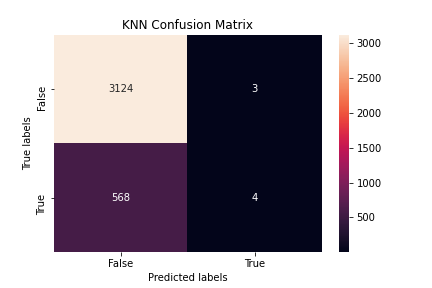
\includegraphics[scale=0.4]{KNN_confusionMatrix.png}
\caption{KNN}
\label{fig:knnMatrix}
\end{subfigure}%
\begin{subfigure}{.5\linewidth}
\centering
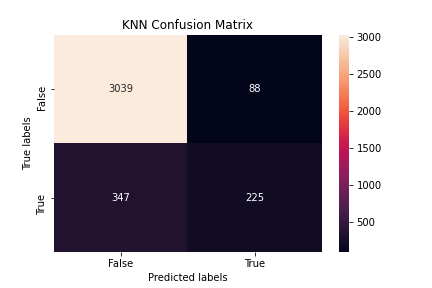
\includegraphics[scale=0.4]{SVM_confusionMatrix.png}
\caption{SVM}
\label{fig:svmMatrix}
\end{subfigure}\\[1ex]
\begin{subfigure}{.5\linewidth}
\centering
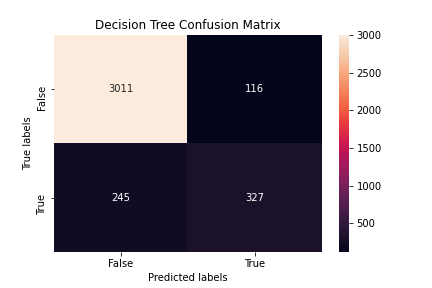
\includegraphics[scale=0.4]{DecisionTree_confusionMatrix.png}
\caption{Decision Tree}
\label{fig:dtMatrix}
\end{subfigure}%
\begin{subfigure}{.5\linewidth}
\centering
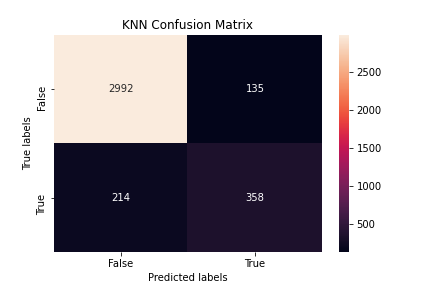
\includegraphics[scale=0.4]{RandomForest_confusionMatrix.png}
\caption{Random Forest}
\label{fig:rfMatrix}
\end{subfigure}\\[1ex]
\caption{Confusion Matrices for Classifiers (with highest weighted F1-Score)}
\label{fig:confusionMatrix}
\end{figure}

\begin{table}[H]
\centering
\begin{tabular}{| c || c | c | c | c | c | c | c | c | c |} 
\hline 
 Model & Accuracy & \multicolumn{2}{|c|}{F1-Score} & \multicolumn{2}{|c|}{Recall} & \multicolumn{2}{|c|}{Precision} & AUROC & AUC-PR \\ \hline
 &  & Macro & Weighted & M & W & M & W & &    \\ \hline 
\hline\hline
KNN &  \cellcolor{red!25}0.8443 & \cellcolor{red!25}0.4615 & \cellcolor{red!25}0.7751 & \cellcolor{red!25}0.5009 & \cellcolor{red!25}0.8442 & \cellcolor{red!25}0.5680 & \cellcolor{red!25}0.7597 & \cellcolor{red!25}0.6038 & \cellcolor{red!25}0.2148  \\ \hline 
SVM & 0.8782 & 0.7038 & 0.8608 & 0.6660 & 0.8782 & 0.8019 & 0.8645 & 0.7789 & 0.5114  \\ \hline 
DT &  0.8939 & 0.7810 & 0.8895 & 0.7630 & 0.8939 & 0.8095 & 0.8890 & 0.9209 & 0.7027  \\ \hline 
RF &  \cellcolor{green!25}0.9031 & \cellcolor{green!25}0.8010 & \cellcolor{green!25}0.8994 & \cellcolor{green!25}0.7810 & \cellcolor{green!25}0.9031 & \cellcolor{green!25}0.8268 & \cellcolor{green!25}0.8979 & \cellcolor{green!25}0.9333 & \cellcolor{green!25}0.7532  \\ \hline 
\end{tabular}
\caption{Average Scores over 10 Models per Classifier}
\label{tab:scores}
\end{table}

\subsection{ROC and PR Curves (d)}

\begin{figure}[H]
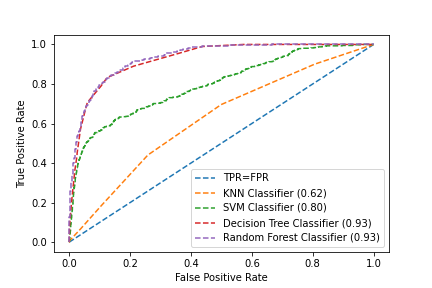
\includegraphics[width=0.90\textwidth]{ROCCurve}
\caption{ROC Curve for Classifiers (with highest F1-Score)}
\label{fig:rocCurve}
\end{figure}

\begin{figure}[H]
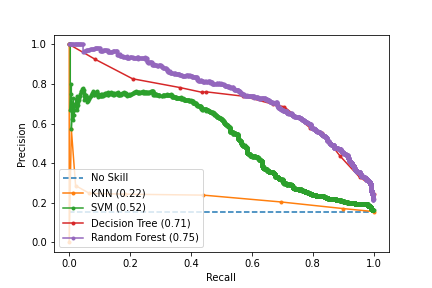
\includegraphics[width=0.90\textwidth]{PRCurve}
\caption{Precision-Recall Curve for Classifiers (with highest F1-Score)}
\label{fig:prCurve}
\end{figure}

\section{Experimental Results from Oversampling (e)}

\subsection{Confusion Matrices and F1-Scores (c)}

\begin{figure}[H]
\begin{subfigure}{.5\linewidth}
\centering
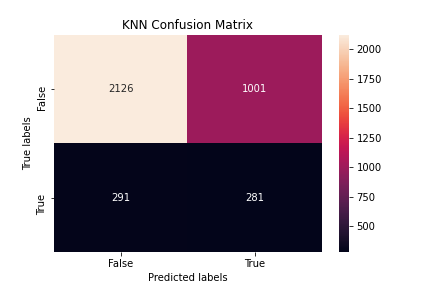
\includegraphics[scale=0.4]{KNN_over_confusionMatrix.png}
\caption{KNN}
\label{fig:knnMatrix_over}
\end{subfigure}%
\begin{subfigure}{.5\linewidth}
\centering
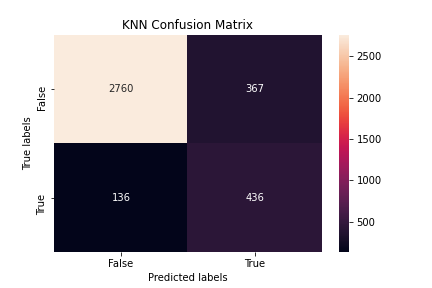
\includegraphics[scale=0.4]{SVM_over_confusionMatrix.png}
\caption{SVM}
\label{fig:svmMatrix_over}
\end{subfigure}\\[1ex]
\begin{subfigure}{.5\linewidth}
\centering
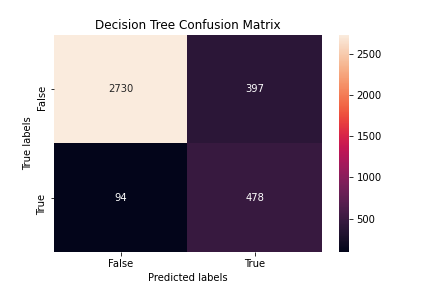
\includegraphics[scale=0.4]{DecisionTree_over_confusionMatrix.png}
\caption{Decision Tree}
\label{fig:dtMatrix_over}
\end{subfigure}%
\begin{subfigure}{.5\linewidth}
\centering
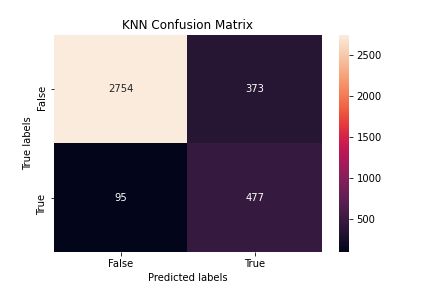
\includegraphics[scale=0.4]{RandomForest_over_confusionMatrix.png}
\caption{Random Forest}
\label{fig:rfMatrix_over}
\end{subfigure}\\[1ex]
\caption{Confusion Matrices for Classifiers (with highest F1-Score), with Oversampling}
\label{fig:confusionMatrix_over}
\end{figure}

\begin{table}[H]
\centering
\begin{tabular}{| c || c | c | c | c | c | c | c | c | c |} 
\hline 
 Model & Accuracy & \multicolumn{2}{|c|}{F1-Score} & \multicolumn{2}{|c|}{Recall} & \multicolumn{2}{|c|}{Precision} & AUROC & AUC-PR \\ \hline
 &  & Macro & Weighted & M & W & M & W & &    \\ \hline 
\hline\hline
KNN &  \cellcolor{red!25}0.6401 & \cellcolor{red!25}0.5252 & \cellcolor{red!25}0.6868 & \cellcolor{red!25}0.5741 & \cellcolor{red!25}0.6406 & \cellcolor{red!25}0.5424 & \cellcolor{red!25}0.7723 & \cellcolor{red!25}0.6051 & \cellcolor{red!25}0.2242  \\ \hline 
SVM & 0.8424 & 0.7501 & 0.8549 & 0.8068 & 0.8424 & 0.7240 & 0.8805 & 0.8878 & 0.6182  \\ \hline 
DT &  0.8547 & 0.7747 & 0.8674 & \cellcolor{green!25}0.8471 & 0.8547 & 0.7427 & 0.8971 & 0.9170 & 0.6891  \\ \hline 
RF & \cellcolor{green!25}0.8690 & \cellcolor{green!25}0.7883 & \cellcolor{green!25}0.8786 & 0.8465 & \cellcolor{green!25}0.8690 & \cellcolor{green!25}0.7573 & \cellcolor{green!25}0.8992 & \cellcolor{green!25}0.9323 & \cellcolor{green!25}0.7449  \\ \hline 
\end{tabular}
\caption{Average Scores over 10 Models per Classifier, with Oversampling}
\label{tab:scores_over}
\end{table}

\subsection{ROC and PR Curves (d)}

\begin{figure}[H]
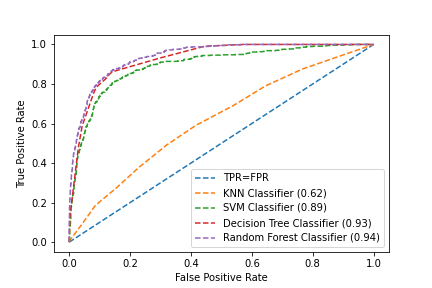
\includegraphics[width=0.90\textwidth]{ROCCurve_over}
\caption{ROC Curve for Classifiers (with highest F1-Score), with Oversampling}
\label{fig:rocCurve_over}
\end{figure}

\begin{figure}[H]
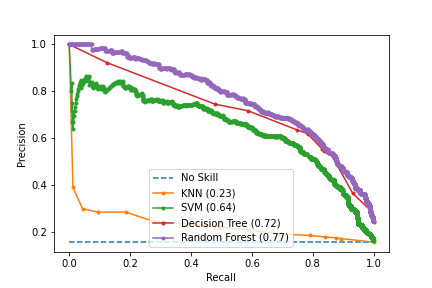
\includegraphics[width=0.90\textwidth]{PRCurve_over}
\caption{Precision-Recall Curve for Classifiers (with highest F1-Score), with Oversampling}
\label{fig:prCurve_over}
\end{figure}

\section{Experimental Results from Undersampling (f)}

\subsection{Confusion Matrices and F1-Scores (c)}

\begin{figure}[H]
\begin{subfigure}{.5\linewidth}
\centering
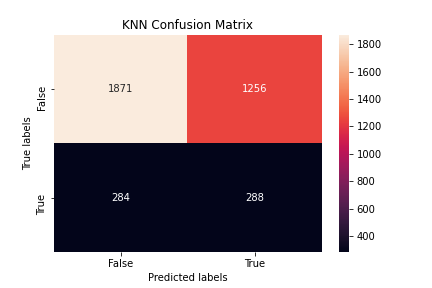
\includegraphics[scale=0.4]{KNN_under_confusionMatrix.png}
\caption{KNN}
\label{fig:knnMatrix_under}
\end{subfigure}%
\begin{subfigure}{.5\linewidth}
\centering
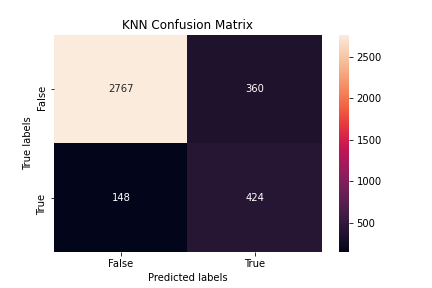
\includegraphics[scale=0.4]{SVM_under_confusionMatrix.png}
\caption{SVM}
\label{fig:svmMatrix_under}
\end{subfigure}\\[1ex]
\begin{subfigure}{.5\linewidth}
\centering
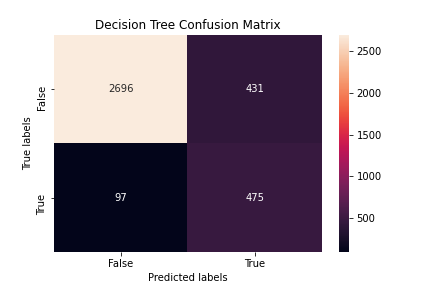
\includegraphics[scale=0.4]{DecisionTree_under_confusionMatrix.png}
\caption{Decision Tree}
\label{fig:dtMatrix_under}
\end{subfigure}%
\begin{subfigure}{.5\linewidth}
\centering
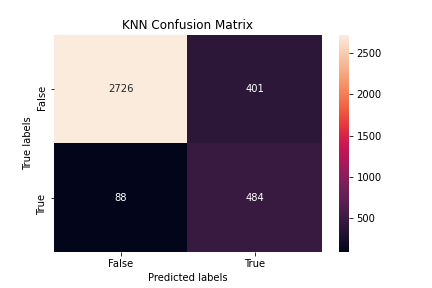
\includegraphics[scale=0.4]{RandomForest_under_confusionMatrix.png}
\caption{Random Forest}
\label{fig:rfMatrix_under}
\end{subfigure}\\[1ex]
\caption{Confusion Matrices for Classifiers (with highest F1-Score), with Undersampling}
\label{fig:confusionMatrix_under}
\end{figure}

\begin{table}[H]
\centering
\begin{tabular}{| c || c | c | c | c | c | c | c | c | c |} 
\hline 
 Model & Accuracy & \multicolumn{2}{|c|}{F1-Score} & \multicolumn{2}{|c|}{Recall} & \multicolumn{2}{|c|}{Precision} & AUROC & AUC-PR \\ \hline
 &  & Macro & Weighted & M & W & M & W & &    \\ \hline 
\hline\hline
KNN &  \cellcolor{red!25}0.5651 & \cellcolor{red!25}0.4850 & \cellcolor{red!25}0.6251 & \cellcolor{red!25}0.5602 & \cellcolor{red!25}0.5651 & \cellcolor{red!25}0.5318 & \cellcolor{red!25}0.7682 & \cellcolor{red!25}0.5851 & \cellcolor{red!25}0.1980  \\ \hline 
SVM &  0.8507 & 0.7584 & 0.8615 & 0.8102 & 0.8507 & 0.7321 & 0.8830 & 0.8858 & 0.6284  \\ \hline 
DT &  0.8453 & 0.7660 & 0.8600 & 0.8470 & 0.8453 & 0.7347 & 0.8962 & 0.9171 & 0.6789  \\ \hline 
RF &  \cellcolor{green!25}0.8570 & \cellcolor{green!25}0.7798 & \cellcolor{green!25}0.8699 & \cellcolor{green!25}0.8567 & \cellcolor{green!25}0.8570 & \cellcolor{green!25}0.7468 & \cellcolor{green!25}0.9011 & \cellcolor{green!25}0.9334 & \cellcolor{green!25}0.7346  \\ \hline 
\end{tabular}
\caption{Average Scores over 10 Models per Classifier, with Undersamping}
\label{tab:scores_under}
\end{table}

\subsection{ROC and PR Curves (d)}

\begin{figure}[H]
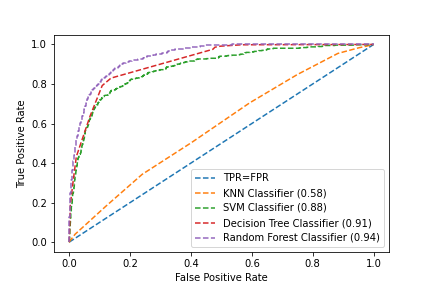
\includegraphics[width=0.90\textwidth]{ROCCurve_under}
\caption{ROC Curve for Classifiers (with highest F1-Score), with Undersampling}
\label{fig:rocCurve_under}
\end{figure}

\begin{figure}[H]
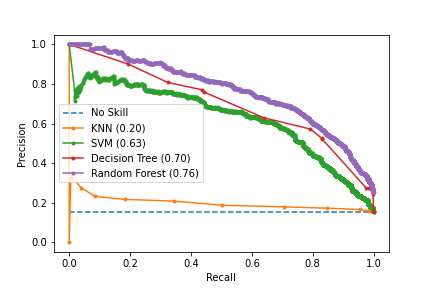
\includegraphics[width=0.90\textwidth]{PRCurve_under}
\caption{Precision-Recall Curve for Classifiers (with highest F1-Score), with Undersampling}
\label{fig:prCurve_under}
\end{figure}

\newpage
\section{Discussion}

\subsection{Best Models (g)}

In each of the three experiments (no resampling, oversampling, and undersampling), the \textbf{Random Forest} models had the best performance. Referring to Tables \ref{tab:scores}, \ref{tab:scores_over}, and \ref{tab:scores_under}, we see that the Random Forest classifier outperformed all of the other models, in virtually all of the metrics. Following from the ROC curves (Figures \ref{fig:rocCurve}, \ref{fig:rocCurve_over}, and \ref{fig:rocCurve_under}) and the PR curves (Figures \ref{fig:prCurve}, \ref{fig:prCurve_over}, and \ref{fig:prCurve_under}), the Random Forest has the highest AUROC and AUC-PR values.

The second best model was the Decision Tree. These results were very close but just bellow those for Random Forest. With a bit more restrictive rounding, we could say that the Decision Tree and Random Forest have basically the same performance, in all of the metrics.

The next best classifier is the SVM classifier. Although the performance is very comparable to that of the Decision Tree and Random Forest, the  SVM classifier took hours to train, whereas all other models took minutes (refer to Table \ref{tab:time}). This information is not negligible, especially in the case of needing real-time training and predictions, as in the reference paper. For this reason, I would not consider this model the best.

The worst classifier, by far, was the KNN algorithm. Even after parameter tuning, this algorithm may be too simple for this classification problem, resulting in underfitting. 

\begin{table}[H]
\centering
\begin{tabular}{| c | c | c | c | c |} 
\hline 
  &  &  & Decision  & Random  \\ 
    & KNN & SVM &  Tree &  Forest \\ \hline
\hline\hline
Parameter Tuning &  1 min & \cellcolor{red!25}10 mins & 1 min  & 2 mins  \\ \hline 
Training &  1 min & \cellcolor{red!25}3 hrs & \textless 1 min & 2 mins  \\
(x10) &  & \cellcolor{red!25} & &  \\ \hline 
Training &  1 min & \cellcolor{red!25}5 hrs & \textless 1 min  & 5 mins  \\
(x10, with oversampling) & & \cellcolor{red!25} & &  \\ \hline
Training & 1 min & \cellcolor{red!25}2 hrs & \textless 1 min  & 1 mins  \\
(x10, with undersampling) &  & \cellcolor{red!25} &  & \\ \hline
\end{tabular}
\caption{Approximation of Time Taken for Different Algorithms. Training for 10 models per classifier.}
\label{tab:time}
\end{table}

\subsection{Comparison of Results Before and After Balancing (g)}

In general, the ranking of the models did not change before and after resampling. The ranking remains (from best to worst): (1) \textbf{Random Forest}, (2) Decision Tree, (3) SVM, and (4) KNN, for oversampling and undersampling.

The best metrics were achieved when the training set was not resampled upon (refer to Table \ref{table:bestModels}). There was not an improvement in any of the metrics from no resampling to resampling. This may be due to overfitting or underfitting when resampling. The worst results came from undersampling, which is to be expected, since there is less data in the training set for the model to learn from.

\begin{table}[H]
\centering
\begin{tabular}{| c || c || c | c | c | c | c | c |} 
\hline
 Resampling & Best Model & Accuracy & \multicolumn{2}{|c|}{F1-Score}  & AUROC & AUC-PR \\ \hline
  & & & Macro & Weighted  & & \\
\hline\hline
None &  Random Forest & \cellcolor{green!25}0.9031 & \cellcolor{green!25}0.8010 & \cellcolor{green!25}0.8994 & \cellcolor{green!25}0.9333 & \cellcolor{green!25}0.7532  \\ \hline 
Oversampling &  Random Forest & 0.8690 & 0.7883 & 0.8786 & 0.9323 & 0.7449 \\ \hline 
Undersampling &  Random Forest & 0.8570 & 0.7798 & 0.8699 & 0.9334 & 0.7346 \\ \hline 
\end{tabular}
\caption{Best Classifiers, with and without Resampling}
\label{table:bestModels}
\end{table}

\section{Comparison with Reference Paper (h)}

Here I will compare the methods and results of my experiment to that of Sakar's paper\cite{sakar_polat_katircioglu_kastro_2018}.

\subsection{Feature Selection}

In Sakar's paper, the authors also used a filter-based feature selection. Using the mRMR statistic, which aims to maximize the relevance between the selected set of features while avoiding redundancy, they ranked the features. This is similar to my correlation matrix method, where I ranked the features based on their correlation to the target feature. My ranking matches the ranking in the 'Correlation' column of their Table 10. I also attempted to reduce redundancy when selecting my top 13 best features, by removing pairs of highly correlated features.

The authors proceed to reduce the feature space by feeding the top 10 features selected by the mRMR filter into a Multi Layer Perceptron (MLP) model, using oversampled data. At the end, they find that including the top 6 features gives the highest possible accuracy and F1-Score:
\begin{itemize}
    \item \emph{PageValue, Month, ExitRates, Weekend, Informational duration, Region}
\end{itemize}

Although our final list of features are not identical, my list does contain their top three features. In comparison, I fed my ranked features into a RandomForest algorithm, and obtained these top 8 features:
\begin{itemize}
    \item \emph{PageValues, ExitRates, ProductRelated, Administrative, VisitorType, Informational, SpecialDay, Month}
\end{itemize}

\subsection{Feature Engineering}

As specified in the assignment instructions, I followed Sakar's procedure for feature engineering: 1-of-C coding of categorical features, and standardization of numerical features. Although they did not provide examples of their transformed features, I would expect our results to be similar.

\subsection{Algorithms and Resampling}

In Sakar's paper, the authors used three main algorithm types: tree-based (Decision Tree and Random Forest), Multi Layer Perceptron, and SVM. They used different hyperparameters for each group of classifiers and obtained accuracies and F1-scores. For each classifier, their training is repeated 100 times with random training/validation partitions.

In my assignment, I used four classifiers: KNN, SVM, Decision Tree, and Random Forest. For each classifier, my training is repeated 10 times with random training/validation partitions. I used hyperparameter tuning on preprocessed data to select the best classification parameters.

For resampling, we both used oversampling of minority class in the training set, while withholding the testing set, to balance the data. Additionally, I attempted undersampling of the majority class.

\subsection{Results}

In the paper, the best F1-score for no resampling and oversampling are obtained with the MLP, with 20 and 10 neurons in the hidden layer, respectively (refer to Table \ref{table:comparison}). The authors see significant improvement of the F1-Score after resampling, in all the classifiers. 

Referring to Table \ref{table:bestModels}, I obtained a higher F1-Score than the authors with the Random Forest algorithm than their MLP, for the no resampling case. I obtained slightly higher results with the Random Forest model for the oversampling case as well. There are many factors which could have contributed to this, such as the feature selection (our feature sets were different), the preprocessing methods, and our hyperparameters. 

The authors did not do undersampling, therefore those results could not be compared.

\begin{table}[H]
\centering
\begin{tabular}{| c | c || c | c |} 
\hline Model & Parameters & Accuracy & F1-Score \\
\hline \hline
 \multicolumn{4}{|c|}{No Resampling} \\ \hline
 MLP & \#neurons=20 & 0.8792 & \cellcolor{green!25}0.58 \\ \hline
 Tree-Based & Random Forest & \cellcolor{green!25}0.8951 & 0.58 \\ \hline
 SVM & kernel=rbf & 0.8614 & 0.53 \\ \hline
 \multicolumn{4}{|c|}{Oversampling} \\ \hline
 MLP & \#neurons=10 & \cellcolor{green!25}0.8724 & \cellcolor{green!25}0.86 \\ \hline
 Tree-Based & C4.5 & 0.8234 & 0.82 \\ \hline
 SVM & kernel=RBF & 0.8488 & 0.82 \\ \hline
\end{tabular}
\caption{Sakar's Best Classification Results\cite{sakar_polat_katircioglu_kastro_2018}}
\label{table:comparison}
\end{table}

\section{Conclusion}

In conclusion, I was able to get good results for this classification problem. First the feature set was preprocessed through feature selection, and feature transformations. Then, I used parameter tuning to select the best hyperparameters for training. Following training, I obtained different metrics for comparing the models, as well as the ROC and PR curves. I also attempted resampling methods to see if this would result in better predictions. In each case (no resampling, oversampling, and undersampling), the Random Forest classifier had the best metrics. Resampling did not improve my F1-scores. My classification results were very slightly higher than those obtained in Sakar's paper.

\newpage
\section{References}
\printbibliography[heading=none]
\newpage

\appendix
\section{Feature Selection}
\label{app:part1}

\begin{figure}[h!]
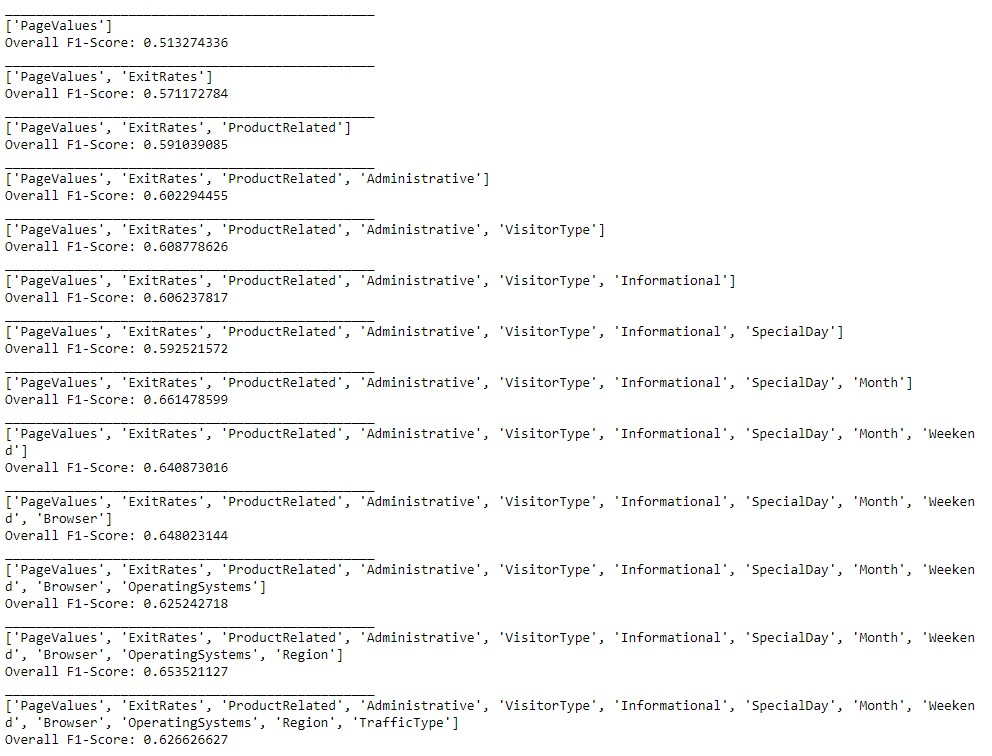
\includegraphics[width=0.95\textwidth]{featureSelectionF1Score}
\caption{F1-Scores of Random Forest Classification, for the purpose of feature selection.}
\label{fig:featureSelection}
\end{figure}
 

\end{document}
